\documentclass[11pt]{article}
\usepackage[utf8]{inputenc}
\usepackage{algorithm}
\usepackage{graphicx}
\usepackage{mathtools}
\usepackage{amsfonts}
\usepackage{hyperref}
\usepackage{geometry}
\usepackage{multicol}
\usepackage{capt-of}
\usepackage{url}
\usepackage[italian]{babel}
\geometry{a4paper, top=2.5cm, bottom=2.5cm, left=3cm, right=3cm, bindingoffset=5mm}
\usepackage[suftesi]{frontespizio}
\title{Relazione di Laboratorio - Tubo di Kundt}
\author{Gruppo I2: Nicolò Favagrossa\\nicolo.favagrossa@studenti.unimi.it, C.M.:969124,}
\date{\today\\A.A. 2020-2021}

\begin{document}
\maketitle
\tableofcontents
\newpage
\section{Introduzione}
L’obiettivo di questa esperienza è misurare la velocità del suono e confrontare il valore misurato con il valore teorico calcolato. Lo scopo dell'esperienza deve essere raggiunto studiando il comportamento delle onde acustiche all’interno del tubo di Kundt nella configurazione con entrambe le estremità chiuse. Questo è un esperimento acustico ideato dal fisico da cui prende il nome, con la funzione di studiare e visualizzare, tramite figure di polvere e sabbia, le onde prodotte da un’onda acustica che passa all’interno di un tubo. Grazie a questo apparato è possibile misurare ed individuare la posizione dei nodi e dei ventri delle onde stazionarie.

In laboratorio l’esperienza inizia campionando le varie onde stazionarie, ognuna con la propria frequenza di risonanza, ponendo il microfono a diverse posizioni. Successivamente, registrando la frequenza e misurando la lunghezza d’onda campionata, si calcola la velocità del suono. Come esperienza parallela, si è studiata la curva di risonanza di uno dei modi normali di oscillazione per visualizzare l'ampiezza dell'onda in funzione della frequenza. Quello che ci aspettiamo è un andamento di tipo lorentziano. 

A esperienza conclusa bisogna confrontare i valori sperimentali ottenuti con i va-lori attesi calcolati attraverso formule teoriche alternative. Infatti, questa esperienza è caratterizzata dal fatto che la grandezza fisica non è direttamente quantificabile se si fa riferimento alla nostra sola percezione, ma con l’aiuto di determinati strumenti è possibile attuare una descrizione concreta capendo e verificando la compatibilità con la trattazione teorica del sistema in esame. Nell'immagine \ref{ciao} si può osservare schematicamente l'apparato sperimentale\footnote{Fonte: \url{https://upload.wikimedia.org/wikipedia/en/1/10/KundtsTube.svg}}.
\begin{figure}[htp!]
\centering
  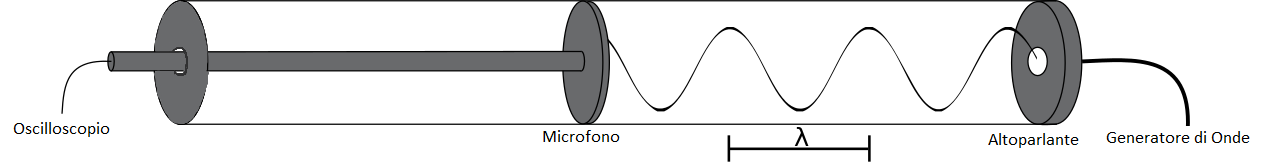
\includegraphics[width=14.5cm]{TuboImmagine.png}\\
  \caption{Un semplice schema per presentare visivamente l'esperienza. Abbiamo il tubo al cui interno passa l'onda acustica. Ad una estremità è presente l'altoparlante collegato al generatore di onde, nell'altra estremità un tappo forato che permette lo scorrimento dell'asta che regge il microfono collegato all'oscilloscopio.}
  \label{ciao}
\end{figure}
\newpage
\section{Trattazione Teorica}
L'oggetto in esame è l'onda acustica. L'equazione che descrive il comportamento di un'onda in funzione dello spazio e del tempo è l'equazione di d'Alambert:
\begin{equation}
    \frac{\partial^2 \psi(x,t)}{\partial t^2} = c^2 \frac{\partial^2 \psi(x,t)}{\partial x^2}
    \label{d'alambert}
\end{equation}
A partire da questa equazione è possibile ricavare la soluzione particolare per le onde stazionarie all'interno di un tubo. La soluzione ha una componente che dipende solo dal tempo e una componente che dipende solo dallo spazio:
\begin{equation}
    \psi(x,t) = A sin\left(\frac{2 \pi}{\lambda}x\right)cos\left(\omega t + \phi\right)
    \label{stazio}
\end{equation}
Da qui definiamo il numero d'onda $k_n=2\pi/\lambda_n$ con $n \in \mathbb{N}$.

Bisogna ora capire il comportamento e le condizioni al contorno del tubo di Kundt con entrambe le estremità chiuse.
All'interno del tubo, in questa specifica configurazione, le particelle d'aria nella posizione $x=0$ e posizione $x=L$ mantengono lo spostamento nullo in quanto presente un tappo che non permette alle particelle di oscillare intorno alla loro posizione di equilibrio. Questo comporta che: $\psi(0,t)=0$ e $\psi(L,t)=0$. Da queste relazione otteniamo che i modi normali di oscillazione, analogamente ad una corda lunga L fissata agli estremi, sono quantizzati:
\begin{equation}
    \lambda_n = \frac{\lambda_1}{n} \qquad\qquad \lambda_1 = 2L \qquad\qquad \forall n \in \mathbb{N}
    \label{k}
\end{equation}
Nell'equazione di d'Alambert (\ref{d'alambert}) $c$ rappresenta la velocità di propagazione dell'onda -in questo caso acustica- che per le condizioni adiabatiche in un gas perfetto equivale a:
\begin{equation}
    c=\sqrt{\frac{\gamma k_B T}{m}} \qquad \qquad \gamma=\frac{c^2m}{k_BT}
    \label{velocità}
\end{equation}
Dove $\gamma = 1.4$ rappresenta il coefficiente di dilatazione adiabatica per i gas biatomici, $k_B = 1.38\times 10^{-23}JK^{-1}$ è la costante di Boltzmann ed $m = 4.7808\times 10^{-26} kg$ è la massa molecorale media del gas in cui l'onda si propaga -l'aria- che per una coerente approssimazione possiamo associarlo ad un gas biatomico. La temperatura all'interno del laboratorio era di $T = (20.02\pm 0.1)^{\circ}C = (293.17\pm 0.1)^{\circ}K$ espressa in gradi Kelvin.
Grazie a questi dati e alla formula (\ref{velocità}) è ora possibile calcolare la velocità del suono all'interno del tubo: $c = (344.202\pm 0.06 )ms^{-1}$.
L'incertezza della velocità è stata ricavata tramite la formula generale della propagazione degli errori, ottenendo:
\begin{equation}
    \sigma_c=\frac{\sqrt{\gamma k_B m T}}{2mT}\sigma_T
\end{equation}

Per ricavare le frequenze dei modi normali di oscillazione si usa la seguente formula:
\begin{align}
    c=\lambda\nu \label{fondamentale} \qquad\qquad \\ 
    \nu_n=\frac{c}{\lambda_n} \label{frequenza} \qquad \forall n \in \mathbb{N}
\end{align}

In questo modo abbiamo le frequenze di risonanza teoriche.
\newpage
\section{Metodi e Materiali}
\subsection{Materiali}
I materiali utilizzati durante l'esperienza sono:

\begin{multicols}{2}
\begin{itemize}
\item Tubo di Plexiglass;
    \item asta rigida;
    \item microfono;
    \item altoparlante;
    \item tappo forato;
    \item morsetti;
    \item metro a nastro;
    \item termometro;
    \item oscilloscopio;
    \item generatore di onde;
    \item connetori per segnali di tipo BNC;
    \item adattatore a "T".
\end{itemize}
\end{multicols}
La configurazione sperimentale è composta da: un tubo di plexiglass in cui viene fatta passare l'onda acustica e un microfono attaccato all'estremità di un'asta rigida poggiata su un tappo forato di gomma che permette all'asta di scivolare liberamente all'interno del tubo.
All'estremità dell'asta sono stati attaccati tre sostegni per fare in modo che il microfono rimanga al centro del tubo e non scorra a contatto diretto con le pareti in plexiglass.
Il microfono, sollecitato dalla variazione di pressione, trasforma il segnale in un segnale elettrico.
Nell'altra estremità del tubo è presente un'altoparlante che trasmette l'onda acustica al suo interno. Il suono è prodotto da un solenoide, una bobina posizionata all'interno di un campo magnetico che spostandosi molto velocemente trascina con sè la membrana dell'altoparlante che oscilla producendo una perturbazione sonora.
L'intera configurazione è retta da due morsetti allineati che mantengono il tubo fisso.

Lungo il tubo è posizionato un metro a nastro che utilizza il centimetro come unità di misura, ha una portata massima di 2 m e una sensibilità di 0.001 m. Il metro serve a misurare la lunghezza del tubo e la posizione di campionamento dell'onda.
In laboratorio è anche presente un termometro con una sensibilità di $0,01^{\circ}C$ per misurare la temperatura dell'aria.
Per riuscire a registrare il suono dal microfono è necessario collegarlo ad un oscilloscopio. Grazie a quest'ultimo strumento si può visualizzare ma anche misurare le ampiezze delle onde.
Equivalentemente l'altoparlante non può funzionare da solo, infatti va collegato ad un generatore di segnali elettrici con frequenza e ampiezza controllabile. Il generatore che abbiamo usato ha un range di: 0,005Hz-5MHz.
L'oscilloscopio è collegato al microfono e il generatore di onde è collegato all'altoparlante tramite dei connetori per segnali di tipo BNC (Bayonet Neill Concelman). 
Per riuscire a visualizzare anche la forma d'onda della forzante è stato necessario utilizzare un adattatore a "T" per riuscire a collegare simultaneamente l'altoparlante e l'oscilloscopio alla stessa uscita del generatore di funzioni.
\subsection{Metodi}
Attraverso il metro a nastro si effettua la misurazione della lunghezza del tubo. Durante la misura bisogna stare attenti ad escludere le porzioni di tappo che servono a mantenerlo aderente al tubo e quindi non misurare l'intera lunghezza. Successivamente attraverso la formula (\ref{k}), si calcolano le prime sei lunghezze d'onda corrispondenti ai primi sei modi normali. Una volta ottenute le lunghezze d'onda e successivamente calcolata la velocità di propagazione con la relazione (\ref{velocità}) è possibile ricavare le frequenze associate con la formula (\ref{frequenza}).

A seguire bisogna determinare sperimentalmente i valori per cui si osservano condizioni di risonanza, per poi confrontarli con i valori attesi. Il primo passo è usare il generatore di onde per riprodurre un'onda con la frequenza calcolata della prima armonica. Fatto ciò è compito dello sperimentatore spostare il microfono lungo il tubo per trovare la posizione dei nodi e ventri. Conoscendo la descrizione teorica ci si aspetta che, per esempio, nel primo modo normale sia presente un solo nodo centrale e per il secondo due nodi rispettivamente a un quarto e  tre quarti della lunghezza del tubo. Quindi, dopo aver verificato la compatibilità del modello atteso, bisogna spostare il microfono all'interno del tubo dove si visualizza un'ampiezza maggiore dall'oscilloscopio. Una volta raggiunta la posizione di massima ampiezza si varia la frequenza prima per eccesso e poi per difetto dal generatore per verificare se la frequenza calcolata è effettivamente la frequenza di risonanza. Nel caso in cui l'ampiezza aumentasse significherebbe che la frequenza calcolata non corrisponde alla frequenza sperimentale. Bisogna eseguire quest'ultimo punto fino a quando non si trova una nuova frequenza che corrisponde alla reale frequenza di risonanza sperimentale. Questo processo va effettuato per tutte le sei armoniche.

Dopo aver misurato le frequenze sperimentali di risonanza è possibile campionare il profilo d'onda del primo modo normale a scelta. La scelta dell'armonica di cui si vuole campionare l'andamento non deve essere casuale, infatti bisogna scegliere modi normali di oscillazioni in cui preferibilmente ci siano più ventri e nodi per favorire lo studio dell'andamento dell'onda e ricavare in maniera più accurata la lunghezza d'onda. Coerentemente, abbiamo scelto di campionare la quarta e la quinta armonica.
Il processo di campionamento inizia con il posizionare il microfono all'inizio del tubo e misurare la posizione con l'ausilio del metro a nastro collocato lungo l'apparato sperimentale di plexiglass. Per quanto riguarda la frequenza di campionamento abbiamo deciso di campionare l'onda ogni 2 o 3 cm aumentanto la frequenza nell'intorno dei nodi per far sì che non ci siano ambiguità durante la misura della lunghezza d'onda. Il campionamento consiste nel misurare l'ampiezza dell'onda in diverse posizioni del microfono all'interno del tubo. Per misurare l'ampiezza abbiamo usato una delle molteplici funzionalità dell'oscilloscopio: due cursori orizzontali che permettono di misurare la distanza tra le loro due posizioni. In questo modo, posizionando una barra tangente alla cresta e l'altra barra tangente al ventre è possibile determinare la differenza di potenziale ($\Delta Posizione$) ai capi del microfono misurata dall’oscilloscopio, infatti le ampiezze sono espresse in volt[V]. Questa distanza non corrisponde direttamente all'ampiezza infatti bisogna estrarla tramite la formula (\ref{Amp}). Durante l'utilizzo dei cursori abbiamo riscontrato del rumore bianco che disturbava la misurazione delle ampiezze. Per eliminare il disturbo esterno è possibile entrare nel menu dell'oscilloscopio ed inserire la modalità "media". Infatti il rumore bianco essendo principalmente casuale tende a sparire quando si effettua una media. 
\begin{equation}
    Ampiezza = \frac{\Delta Posizione}{2}
    \label{Amp}
\end{equation}

Alla fine del campionamento, attraveso il grafico delle ampiezze in funzione della posizione abbiamo calcolato la lunghezza d'onda. Partendo dalla quarta armonica abbiamo ricavato la distanza tra i primi due nodi ($D_1$), tra il secondo nodo ed il terzo ($D_2$) e successivamente tra il terzo e quarto nodo ($D_3$), poi abbiamo calcolato la media delle distanze ($\bar{D}$) e ricavato la lunghezza d'onda con la seguente relazione:
\begin{equation}
    \lambda = 2 \bar{D}
\label{distanza}
\end{equation}
Successivamente abbiamo svolto l'analogo processo per la quinta armonica. Ora abbiamo tutte le componenti della formula (\ref{fondamentale}) per calcolare la velocità del suono e successivamente anche il coefficiente di dilatazione adiabatica attraverso la formula (\ref{velocità}).

Nell'ultima parte dell'esperienza, per ricostruire la risposta del sistema in corrispondenza delle frequenze nell'intorno di una condizione di risonanza, abbiamo scelto di studiare il terzo modo normale di oscillazione. Come per lo studio delle onde stazionarie abbiamo utilizzato la configurazione del tubo con entrambe le estremità chiuse per limitare disturbi provenienti dal laboratorio. Come prima cosa abbiamo impostato la frequenza di risonanza misurata sperimentalmente e cercato la posizione del microfono in cui è presente un ventre. Una volta individuato il ventre abbiamo utilizzato nuovamente la funzione dei cursori dell'oscilloscopio per misurare l'ampiezza  dell'onda di risonanza espressa in volt[V]. Dopo aver campionato un numero sufficiente di configurazioni si può ricostruire l'andamento delle ampiezze in funzione della frequenza. Questo andamento, coerentemente con la teoria, deve essere di tipo lorentziano con un massimo centrale e dei minimi simmetrici all'estremità della funzione. 

Durante il campionamento, per ottenere il grafico della fase in funzione della frequenza abbiamo misurato, tramite i cursori verticali, la distanza tra un ventre della forzante ed il ventre successivo dell'onda acustica. La fase è legata al ritardo di un'onda rispetto ad un'altra. Questo ritardo rapportato al periodo dell'onda è la frazione di ciclo trasformato in un angolo di fase. La fase che ci aspettiamo è uno sfasamento di $\frac{\pi}{2}$ nella frequenza di risonanza. Questo risultato è corretto attenderlo per quanto riguarda le grandezze meccaniche. In realtà stiamo misurando dei segnali elettrici che passano attraverso tutta l'elettronica dell'oscilloscopio, perciò bisogna tenere in considerazione che possono esserci degli effetti di sfasamento anche importanti tra il segnale elettrico e la fornzante meccanica.

\section{Risultati Sperimentali}
\subsection{Risultati preliminari}
La lunghezza del tubo è: $L=(0.742\pm0.001)m$.
Da qui riporto la tabella dei risultati ottenuti dalla prima analisi e misurazione:
\begin{table}[H]
    \centering
    \begin{tabular}{|c|c|c|}
    \hline
    $\lambda_{teo}\pm \sigma_\lambda(m):$ & $\nu_{teo}\pm \sigma_\nu(Hz):$ & $\nu_{spe}\pm \sigma_{\nu'}(Hz):$ \\
    \hline
    $1.484\pm0.002$ & $231.942\pm0.315$ & $225\pm0.5$ \\
    \hline
    $0.742\pm0.001$ & $463.884\pm0.63$ & $451\pm0.5$ \\
    \hline
    $0.495\pm0.001$ & $695.826\pm0.945$ & $658\pm0.5$ \\
    \hline
    $0.371\pm0.001$ & $927.767\pm1.284$ & $950\pm0.5$ \\
    \hline
    $0.297\pm0.001$ & $1159.709\pm1.575$ & $1168\pm0.5$ \\
    \hline
    $0.247\pm0.001$ & $1391.651\pm1.89$ & $1393\pm0.5$ \\
    \hline
    \end{tabular}
    \caption{Sono riportate le lunghezze d'onda calcolate tramite la lunghezza del tubo, le frequenze calcolate e le frequenze misurate sperimentalmente. Tutte le misure sono espresse con le proprie incertezze.}
    \label{c}
\end{table}Per calcolare l'incertezza relativa alla lunghezza d'onda abbiamo utilizzato la propa-gazione degli errori per una costante, infatti:
\begin{equation}
    \sigma_\lambda=\frac{2\sigma_L}{n} \qquad n =1,2...,6
\end{equation}
Analogamente per l'incertezza relativa alla frequenza calcolata abbiamo ricavato la formula:
\begin{equation}
    \sigma_\nu=\sqrt{\left(\frac{\sigma_c}{\lambda}\right)^2+\left(\frac{c\sigma_\lambda}{\lambda^2}\right)^2}
\end{equation}
 
\subsection{Quarto modo normale di oscillazione}
Analiziamo i risultati ottenuti dal quarto modo normale di oscillazione. Nel grafico \ref{n4} è possibile visualizzare l'ampiezza dell'onda acustica in funzione della posizione del microfono all'interno del tubo di plexiglass. 
  \begin{figure}[H]
  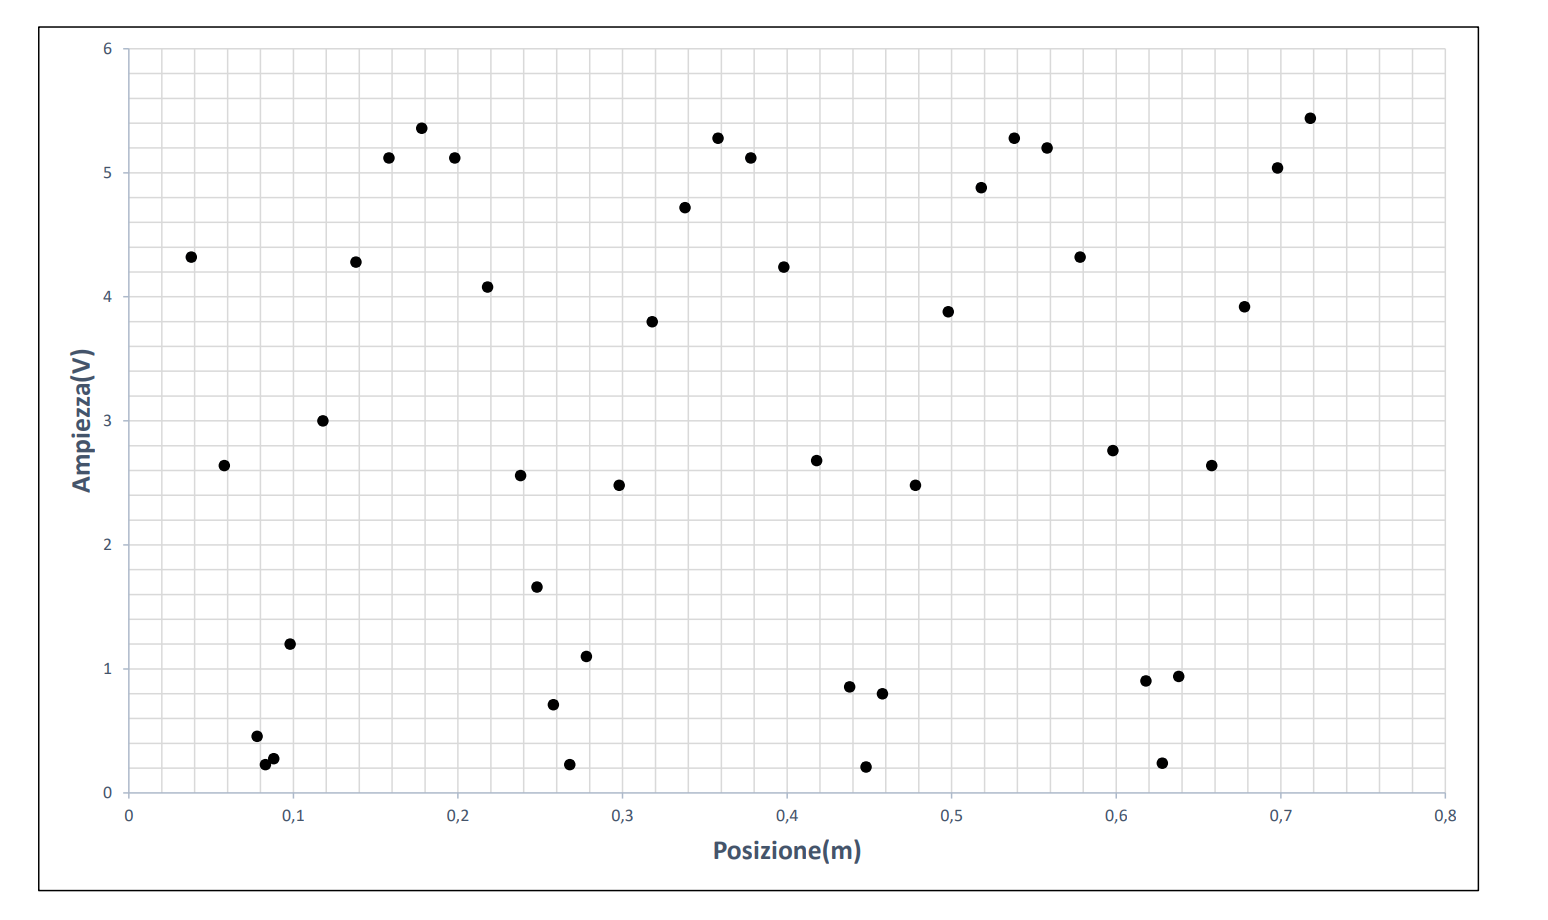
\includegraphics[width=14cm]{Modo Normale 4.png}\\
  \caption{Il grafico rappresenza l'ampiezza dell'onda del quarto modo di oscillazione campionata nelle diverse posizioni del microfono. L'incertezza relativa alla posizione e all'ampiezza è rispettivamente $\sigma_P=0.001m$, $\sigma_A=0.02V$. Le ampiezze sono state campionate ogni 2 cm grazie al quale si può osservare in maniera chiara il profilo dell'onda acustica all'interno del tubo di Kundt.}
  \label{n4}
  \end{figure}

Individuando i nodi presenti sul grafico abbiamo ricavato la distanza: $\bar{D}=(0.182\pm0.002)m$.
Di seguito i risultati ottenuti tramite le formule e i processi descritti in precedenza:
\begin{itemize}
    \item $\lambda_4=(0.363\pm0.002)m$;
    \item $\nu_4=(950\pm0.5)Hz$;
    \item $c=(345.167\pm1.909)ms^{-1}$;
    \item $\gamma=1.408\pm0.016$
\end{itemize}
Abbiamo ricavato l'incertezza della velocità attraverso la formula generale della propa-gazione degli errori:
\begin{equation}
    \sigma_c=\sqrt{(\nu\sigma_{\lambda})^2+(\lambda \sigma_\nu)^2}
    \label{sigmav}
\end{equation}
Analogamente è stata ricavata l'incertezza sul coefficiente di dilatazione adiabatica:
\begin{equation}
    \sigma_\gamma=\sqrt{\left(\frac{mc^2}{k_BT}\right)\sigma_T^2+\left(\frac{2mc}{k_BT}\right)^2\sigma_c^2}
    \label{sigmag}
\end{equation}
\subsection{Quinto modo normale di oscillazione}
Per quanto riguarda il quinto modo normale di oscillazione abbiamo ottenuto dei valori compatibili ma comunque diversi. Il grafico \ref{n5} riporta il profilo d'onda campionato in laboratorio. A differenza del precedente campionamento abbiamo deciso di campionare l'onda ogni 3 cm. Come si può osservare dal grafico questa differenza rende l'andamento meno continuo e chiaro in quanto i punti sono più distanti.
\begin{figure}[H]
\centering
  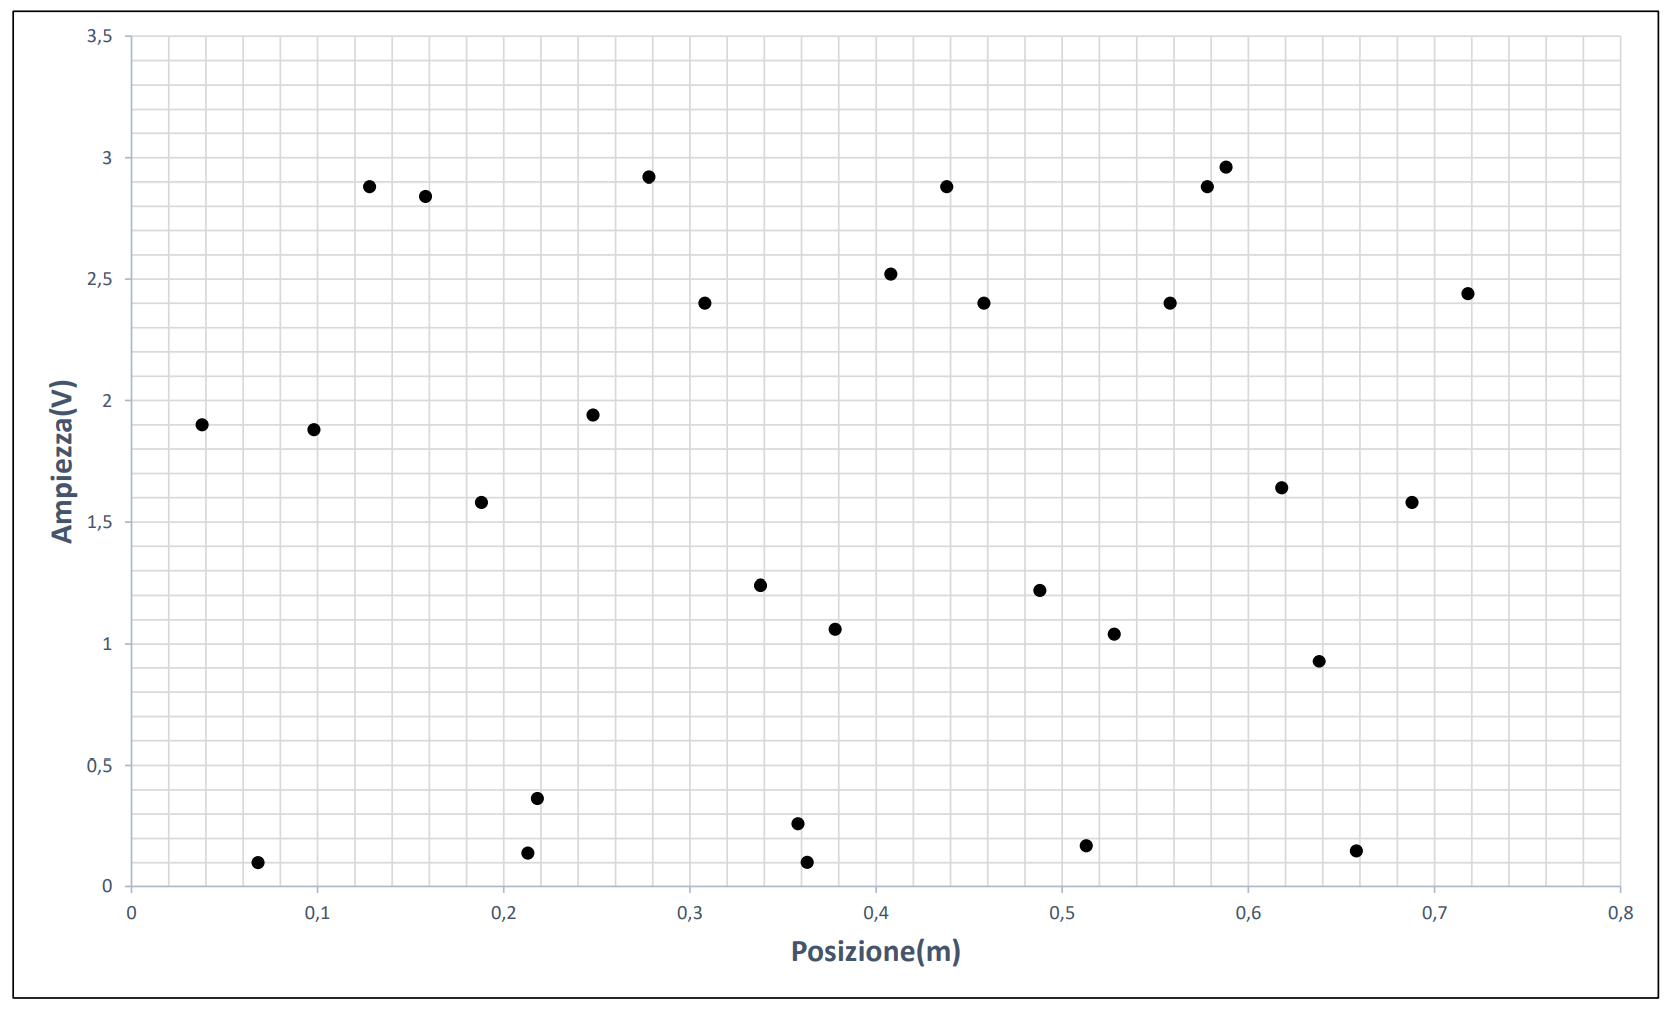
\includegraphics[width=14cm]{Modo Normale 5.png}\\
  \caption{Il grafico rappresenta il profilo d'onda del quinto modo normale di oscillazione. Si può visualizzare l'andamendo delle ampiezze in funzione della posizione del microfono all'interno del tubo. L'incertezza della posizione e dell'ampiezza è rispettivamente $\sigma_P=0.001m$, $\sigma_A=0.02V$.}
  \label{n5}
\end{figure}
Analogamente all'analisi effettuata precedentemente, abbiamo calcolato la distanza tra i cinque nodi dell'onda acustica visualizzabile nel grafico \ref{n5}. $\bar{D}=(0.148\pm0.002)m$.
Per la quinta armonica abbiamo ottenuto i seguenti valori:
\begin{itemize}
    \item $\lambda_5=(0.295\pm0.002)m$;
    \item $\nu_5=(1168\pm0.5)Hz$;
    \item $c=(344.56\pm2.34)ms^{-1}$;
    \item $\gamma=1.403\pm0.019$
\end{itemize}
Le incertezze, sono state calcolate attraverso le medesime formule usate nel quarto modo normale. Quindi abbiamo utilizzato la formula (\ref{sigmav}) per l'incertezza sulla velocità e la formula (\ref{sigmag}) per l'incertezza relativa al coefficiente di dilatazione adiabatica.
\newpage
\subsection{Confronto dei dati ottenuti}
Nell'ipotesi che i dati sperimentali si distribuiscano su una gaussiana è possibile fare un confronto quantitativo
attraverso la formula:
\begin{equation}
    z= \frac{|c_n-c_{teo}|}{\sqrt{\sigma_{cn}^2+\sigma_{cteo}^2}} \qquad n=4,5
    \label{z}
\end{equation}
L'osservabile $z$ per la quarta armonica corrisponde a: $z_4=0.505$. Dopo aver consultato le tabelle appropriate si ricava la probabilità che la misura sia diversa dal valore teorico per fluttuazioni statische. Per il primo risultato abbiamo ottenuto il $61\%$ di probabilità.
Per quanto riguarda la quinta armonica abbiamo ottenuto: $z_5=0.153$ che corrisponde al $88\%$ di probabilità. Di seguito riporto il grafico in cui si possono visualizzare i valori con le relative barre d'incertezza. Alla luce di questi risultati le due misure sono consistenti.
\begin{figure}[H]
\centering
  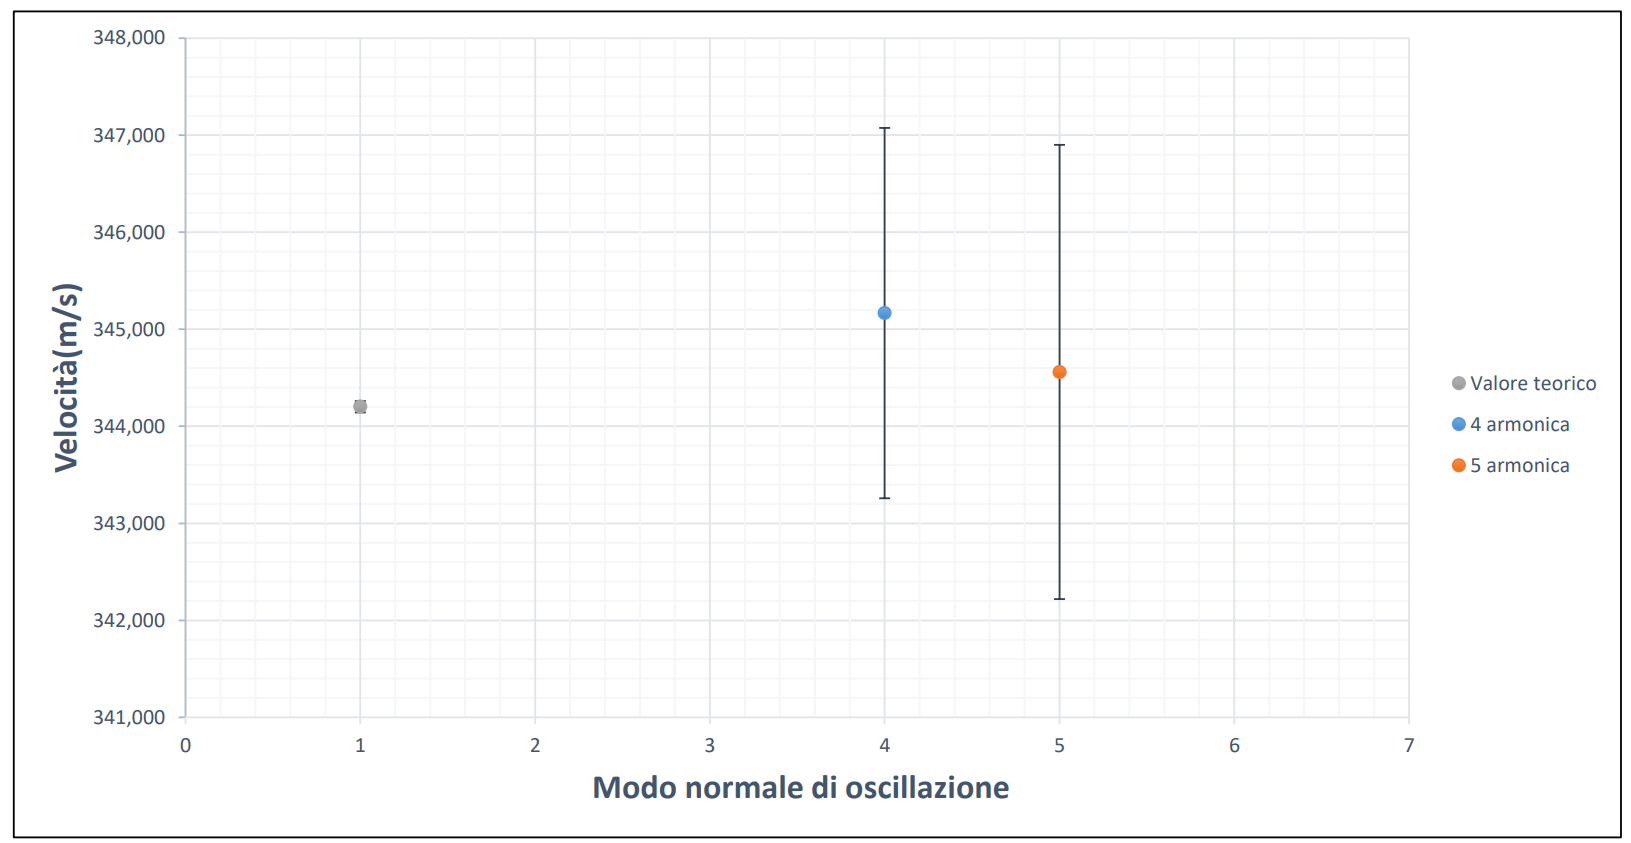
\includegraphics[width=14cm]{Errore.png}\\
  \caption{Il grafico rappresenta la velocità teorica e le due velocità misurate con le barre di errore che corrispondono all'incertezza calcolata precedentemente.}
  \label{Barre}
\end{figure}

\subsection{Risonanza}
Si può osservare dal grafico \ref{ri} un andamento di tipo lorentziano con un picco nella posizione $x=(655\pm0.5)Hz$ che corrisponde alla frequenza di risonanza. Per quanto riguarda l'andamento della fase, attraverso la misura del tempo tra la forzante e l'onda acustica abbiamo ottenuto il grafico \ref{Fase}. Non avendo un valore atteso della larghezza della lorentziana non è stato possibile avere un paragone quantitativo con un modello teorico, ma mettendo a confronto il grafico \ref{ri} e il grafico \ref{Fase} è possibile osservare che il punto di flesso  nel secondo grafico corrisponde al picco della lorentziana del primo grafico. Infatti l'obiettivo di quest'ultima esperienza è di riuscire a visualizzare i due andamenti. Per lo stesso motivo, nel grafico \ref{Fase}, ho deciso di mantenere nelle ordinate il tempo (al posto dei radianti) perchè l'andamento dei vari campionamenti sul grafico rimane invariato per una costante di conversione.

\begin{figure}[H]
\centering
  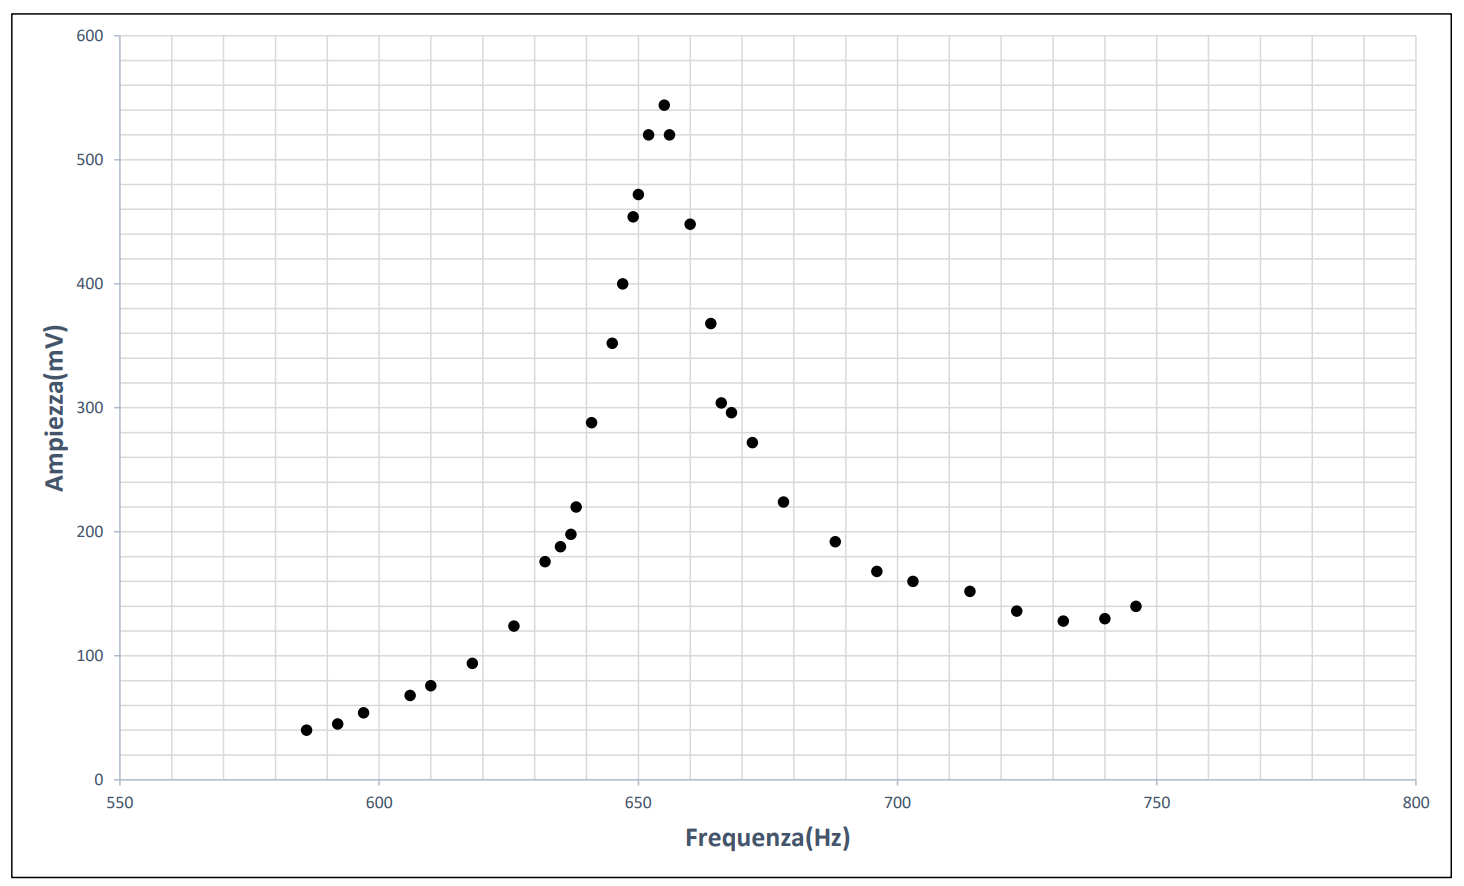
\includegraphics[width=14cm]{Risonanza.png}\\
  \caption{Il grafico rappresenza l'ampiezza misurata come differenza di potenziale in funzione della frequenza in un intorno di risonanza. Si può osservare il caratteristico picco e minimi della lorentziana anche se in questo caso visivamente asimmetrica.}
  \label{ri}
\end{figure}

\begin{figure}[H]
\centering
  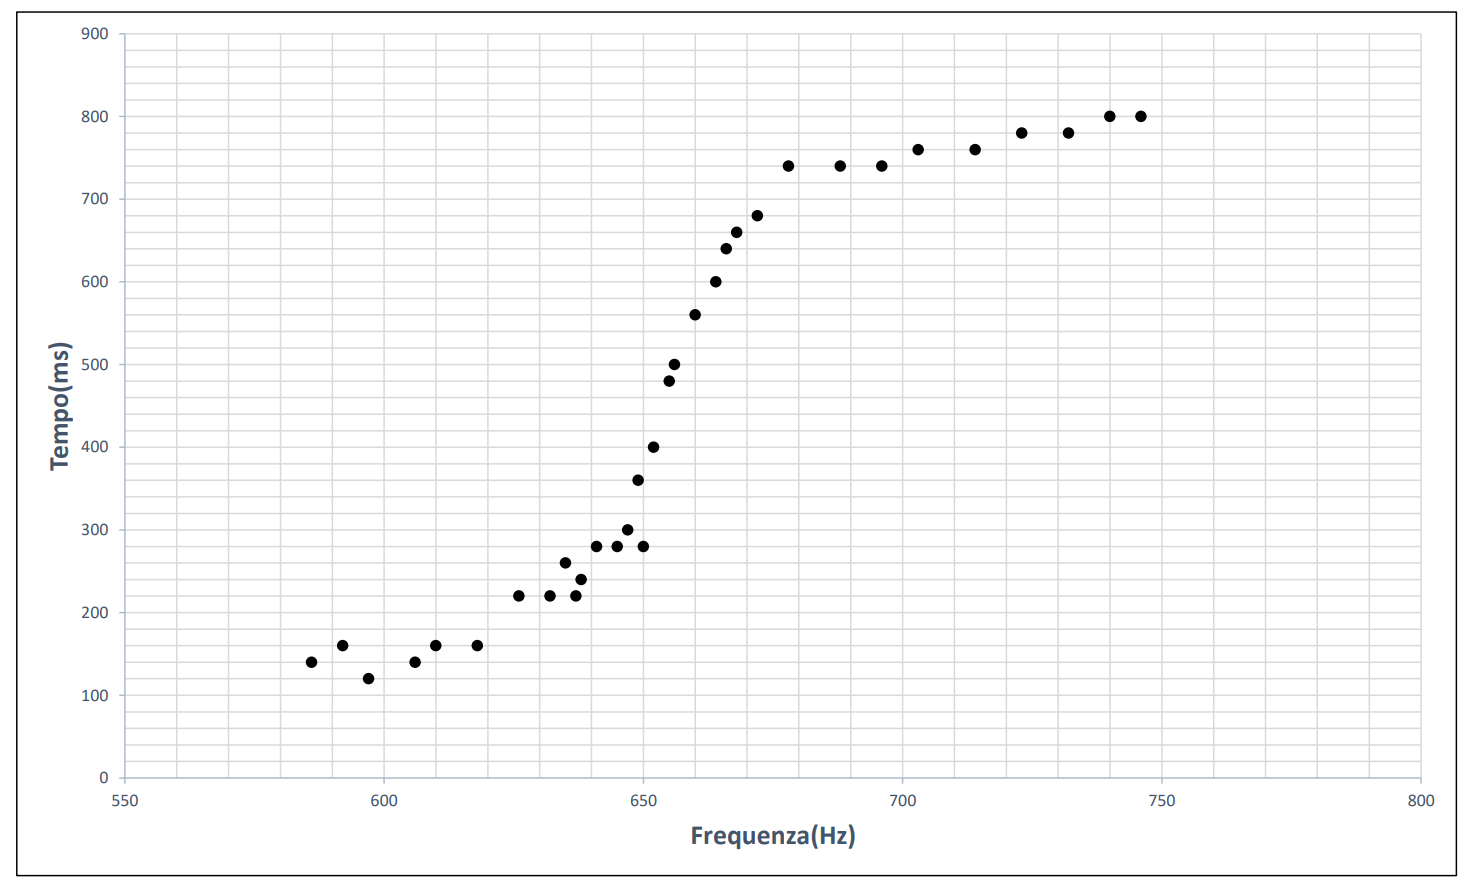
\includegraphics[width=14cm]{FaseT.png}\\
  \caption{Il grafico rappresenta il tempo (in ms) tra la forzante e l'onda acustica in funzione della frequenza. Si può osservare un punto di flesso in corrispondenza di $x=(655\pm0.5)Hz$ che corrisponde alla frequenza di risonanza.}
  \label{Fase}
\end{figure}
\newpage
\section{Conclusione}
Ricapitolando gli obiettivi dell'esperienza sono: misurare la velocità del suono all'inter-no del tubo di Kundt con entrambe le estremità chiuse attraverso misure indirette, calcolare con la velocità misurata il coefficiente di dilatazione adiabatica per i gas biatomici ed infine studiare l'andamento dell'onda acustica in funzione della frequenza di risonanza. Durante l'esperienza abbiamo utilizzato e imparato ad utilizzare diversi strumenti tra cui l'oscilloscopio e il generatore di onde. Abbiamo studiato e ricavato la velocità del suono con due diverse armoniche (la quarta e la quinta armonica) e ottenuto due risultati differenti: $c_4=(345.167\pm1.909)ms^{-1}$  $c_5=(344.56\pm2.34)ms^{-1}$ con le relative costanti adiabatiche: $\gamma_4=1.408\pm0.016$  $\gamma_5=1.403\pm0.019$. I risultati ottenuti sono compatibili con il valore teorico calcolato all'inizio dell'esperienza. La compatibilità infatti è stata studiata ipotizzando che le misure si distribuiscano secondo una gaussiana e quindi calcolando l'osservabile $z$. I valori infatti sono compatibili rispettivamente per il $61\%$ e $88\%$ di probabilità. Per quanto riguarda lo studio del comportamento dell'onda acustica in un intorno della frequenza di risonanza siamo riusciti ad ottenere due grafici che rappresentano il profilo d'onda e l'andamento della fase in funzione della frequenza, visualizzabili rispettivamente nel grafico \ref{ri} e \ref{Fase}. L'unica ambiguità nata durante l'esperienza riguarda la differenza tra le frequenze calcolate e misurate. Infatti per la seconda e la terza armonica abbiamo calcolato una discrepanza tra i valori teorici e sperimentali che supera i $20Hz$. Durante l'esperienza sono stati raggiunti tutti gli obiettivi.
\end{document}

